\documentclass[letterpaper,12pt]{article} % This defines the style of your paper
\usepackage[top = 2.5cm, bottom = 2.5cm, left = 2.5cm, right = 2.5cm]{geometry} 

% The following two packages - multirow and booktabs - are needed to create nice looking tables.
%\usepackage{multirow} % Multirow is for tables with multiple rows within one cell.
%usepackage{booktabs} % For even nicer tables.

% As we usually want to include some plots (.pdf files) we need a package for that.
\usepackage{graphicx} 
\usepackage[export]{adjustbox}

% The default setting of LaTeX is to indent new paragraphs. This is useful for articles. But not really nice for homework problem sets. The following command sets the indent to 0.
\usepackage{setspace}
\setlength{\parindent}{0in}

% Package to place figures where you want them.
%usepackage{float}

% The fancyhdr package let's us create nice headers.
\usepackage{fancyhdr}
\usepackage{amsmath}


\usepackage[
backend=biber,
style=numeric,
citestyle=numeric
]{biblatex}

\addbibresource{references.bib} %Imports bibliography file

%%%%%%%%%%%%%%%%%%%%%%%%%%%%%%%%%%%%%%%%%%%%%%%%
% 3. Header (and Footer)
%%%%%%%%%%%%%%%%%%%%%%%%%%%%%%%%%%%%%%%%%%%%%%%%

% To make our document nice we want a header and number the pages in the footer.

\pagestyle{fancy} % With this command we can customize the header style.

\fancyhf{} % This makes sure we do not have other information in our header or footer.

\lhead{\footnotesize MATH339: Assignment 1}% \lhead puts text in the top left corner. \footnotesize sets our font to a smaller size.

%\rhead works just like \lhead (you can also use \chead)
\rhead{\footnotesize Johns} %<---- Fill in your lastnames.

% Similar commands work for the footer (\lfoot, \cfoot and \rfoot).
% We want to put our page number in the center.
\cfoot{\footnotesize \thepage} 


\begin{document}

%%%%%%%%%%%%%%%%%%%%%%%%%%%%%%%%%%%%%%%%%%%%%%%%
% Title section of the document
%%%%%%%%%%%%%%%%%%%%%%%%%%%%%%%%%%%%%%%%%%%%%%%%

\thispagestyle{empty} % This command disables the header on the first page. 

\begin{tabular}{p{15.5cm}} % This is a simple tabular environment to align your text nicely 
{\large \bf COMP361: Numerical Methods} \\
Concordia \\ Winter 2021 \\ A. Krzyzak \\
\hline % \hline produces horizontal lines.
\\
\end{tabular} % Our tabular environment ends here.

\vspace*{0.3cm} % Now we want to add some vertical space in between the line and our title.

\begin{center} % Everything within the center environment is centered.
	{\Large \bf Assignment 1} % <---- Don't forget to put in the right number
	\vspace{2mm}
	
        % YOUR NAMES GO HERE
	{\bf Amiani Johns 26388620}
		
\end{center}  

\vspace{0.4cm}

%%%%%%%%%%%%%%%%%%%%%%%%%%%%%%%%%%%%%%%%%%%%%%%%
%%%%%%%%%%%%%%%%%%%%%%%%%%%%%%%%%%%%%%%%%%%%%%%%

% Up until this point you only have to make minor changes for every week (Number of the homework). Your write up essentially starts here.

\begin{enumerate}

  \item {
    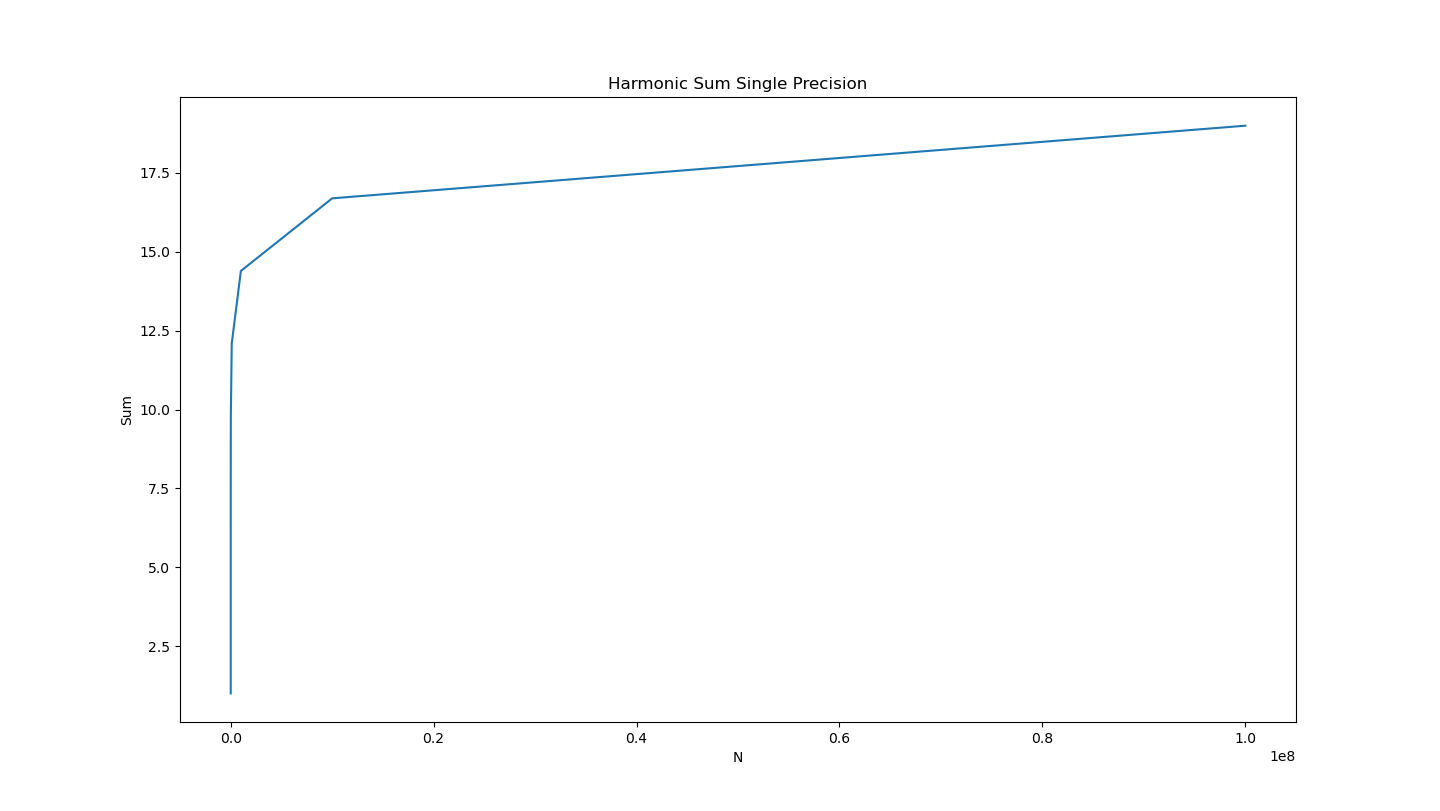
\includegraphics[width=0.5\textwidth, valign=t]{hsumsingle.png}
    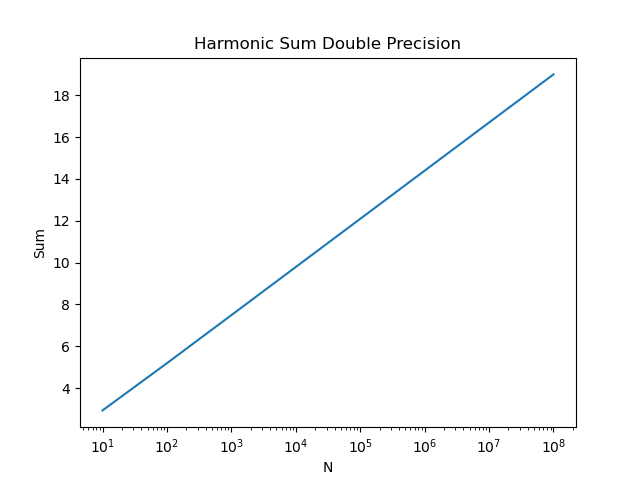
\includegraphics[width=0.5\textwidth, valign=t]{hsumdouble.png}

    Figures 1 and 2 show the behaviour of the harmonic sum for various values of N. Note that the N values are plotted on a log scale. In both plots we see that the sum continues to grow as N increases.

    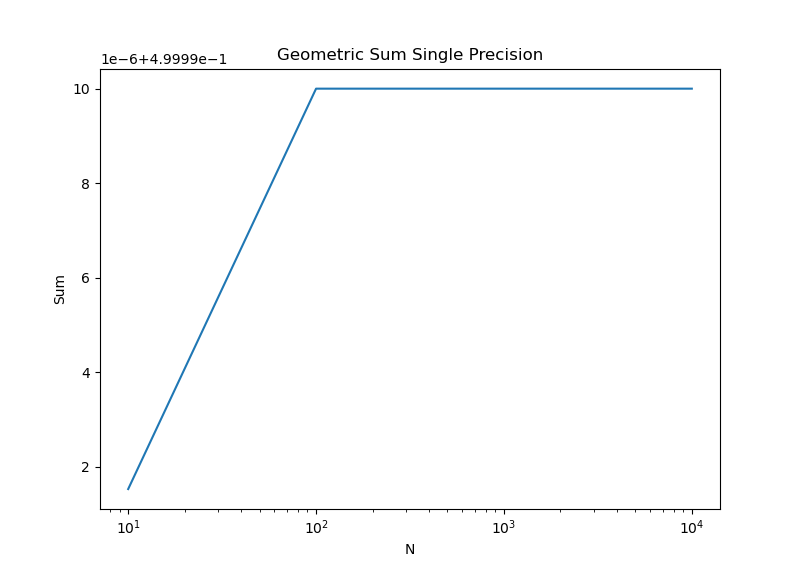
\includegraphics[width=0.5\textwidth]{geosumsingle}
    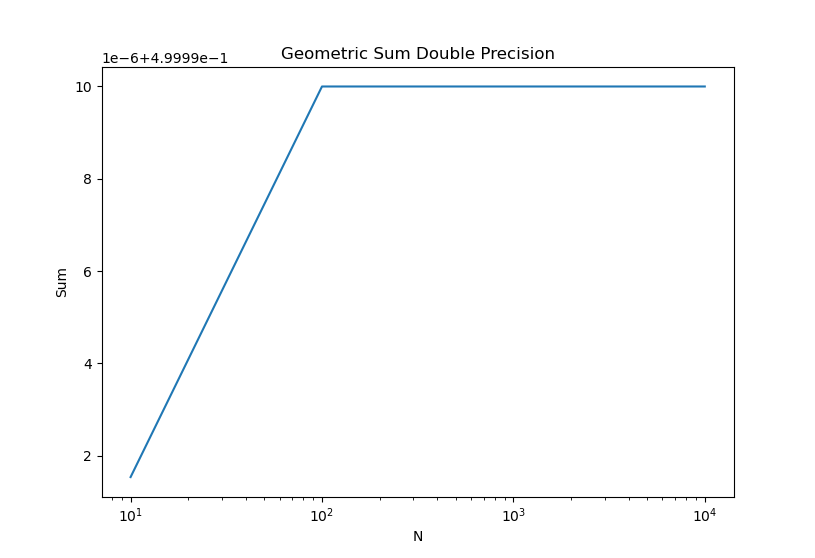
\includegraphics[width=0.5\textwidth]{geosumdouble}
    In both cases the sum has converged when \(N = 100\).\\
    The sum of a geometric series with constant ratio \(r\) less than 1 sum can be calculated using the formula\cite{geoseries}
    \[ \sum_{k=1}^{N} r^k = \frac{r(1-r^N)}{1-r} \]
    Our series has \(r = \frac{1}{3}\), so the sum is
    \[ \frac{\frac{1}{3}(1-(\frac{1}{3})^N)}{1-\frac{1}{3}} = \frac{1}{2} \left( 1-\frac{1}{3^N} \right) \]
    In the limit of large \(N\), the sum of a geometric series with constant ratio less than 1 can be calculated using the formula\cite{geoseries}
    \[ \sum_{k=1}^{\infty} = \frac{r}{1-r} \]
    Which for \(r = \frac{1}{3} \) is \(\frac{1}{2}\).
  }

  \item {
    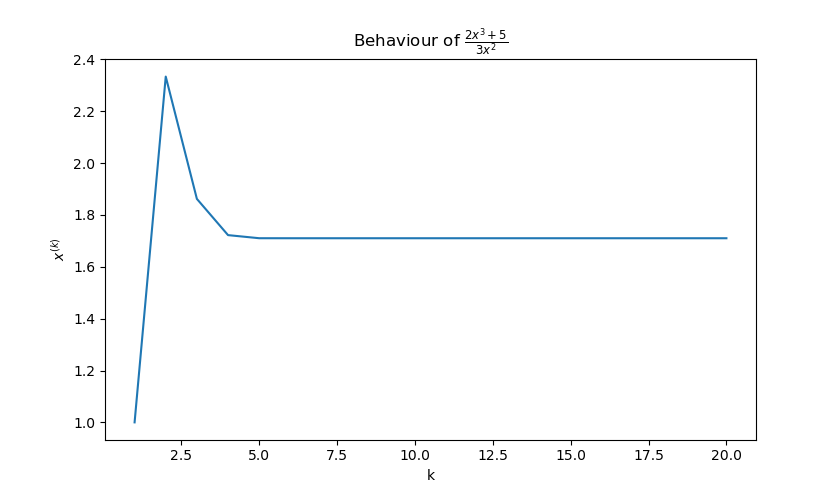
\includegraphics[width=\textwidth, valign=t]{q2seq1}
    We see from the above figure that sequence initially rises before settling to a fixed point \(x^*\) after \(k=5\). We find this fixed point by solving
    \[ x = f(x) \]
    where
    \[ f(x) = \frac{2x^3 + 5}{3x^2} \]
    therefore
    \[ x^* = \sqrt[3]{5} \]
    This fixed point does not depend on \(x^{(0)}\).
    
    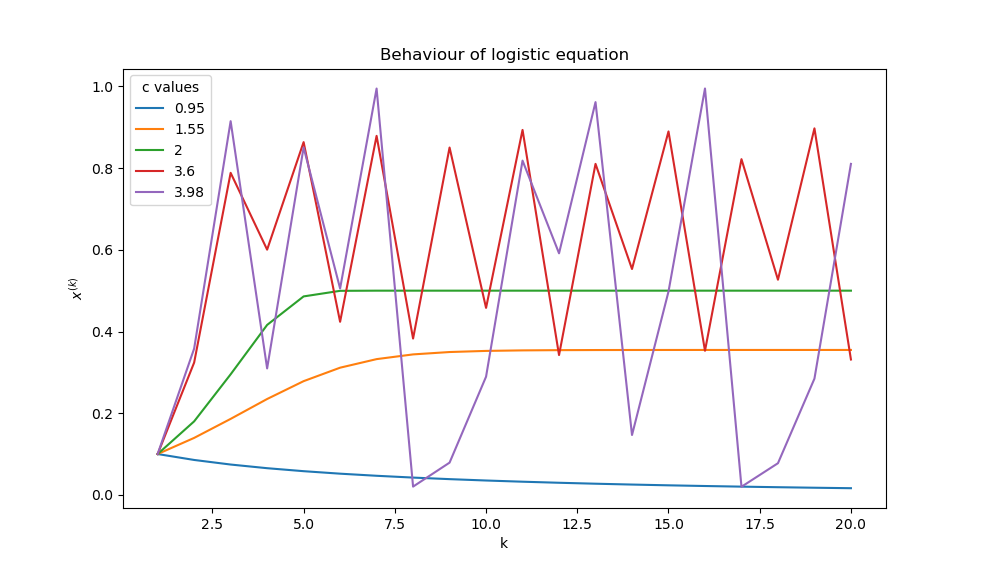
\includegraphics[width=\textwidth]{q2logseq}
    When \(c=0.95\), the sequence is attacted to the fixed point at 0.\\
    When \(c=1.55\), the sequence is attracted to the fixed point at \( 1-\frac{1}{1.55} = 0.355 \).\\
    When \(c=2\), the sequence is attracted to the fixed point at \( 1-\frac{1}{2} = \frac{1}{2} \).\\
    When \(c=3.6\), \(|f'(x^*)| = 1.6 > 1 \), so the sequence is repelled from the fixed point at \( 1-\frac{1}{3.6} = 0.722 \).\\
    When \(c=3.98\), \(|f'(x^*)| = 1.98 > 1 \), so the sequence is repelled from the fixed point at \( 1-\frac{1}{3.98} = 0.749 \).
  }
  
  \item {
    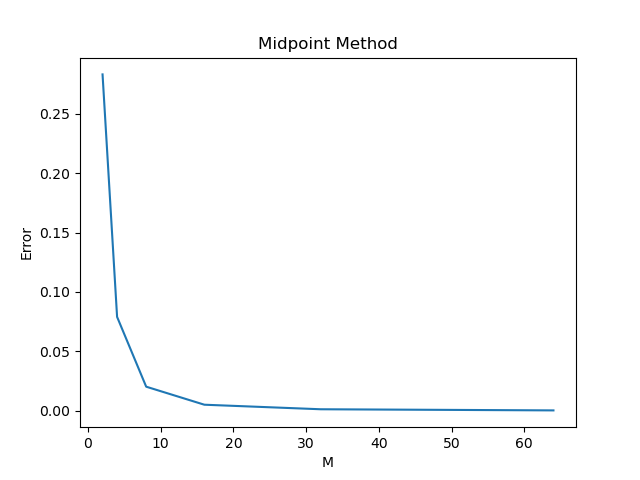
\includegraphics[width=0.5\textwidth, valign=t]{mperror}
    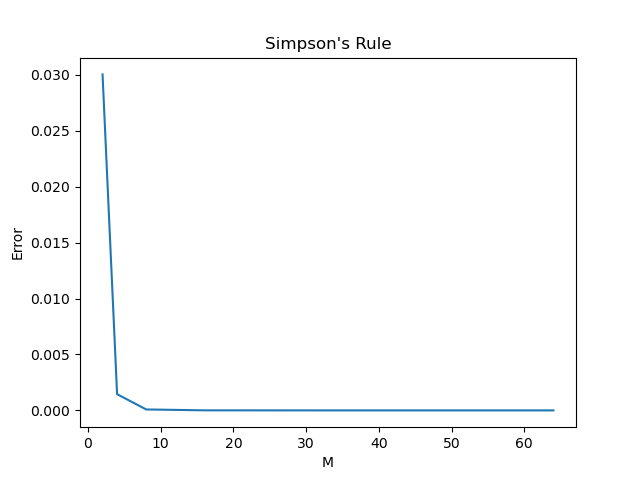
\includegraphics[width=0.5\textwidth, valign=t]{sierror}

    For the Midpoint Method, the smallest \(M\) for which the error is less than \(10^{-7}\) is \(2^{11}\). This corresponds to 2048 function evaluations.\\
    For Simpson's Method, the smallest \(M\) for which the error is less than \(10^{-7}\) is \(2^{6}\). This corresponds to 65 function evaluations.\\

    For both methods, the error decreases sharply with \(h\). As \(M\) gets very large the error tends towards 0.

    \begin{enumerate}
      \newcommand{\norm}[1]{\lVert#1\rVert}
      \item[a)] {
        The error bound for the Midpoint Rule is given by\cite{errorbound}
        \[ |E_M| \leq \norm{f''(x)}_\infty \frac{(b-a)^3}{24M^2} \]
        In our case, \( |f''(x)| = |-\pi^2 \sin(\pi x)| \), which is greatest when the argument to the \(\sin\) term is \(\frac{\pi}{2}\), i.e. at \(x = \frac{1}{2}\). So
        \[ \norm{f''(x)}_\infty = \pi^2 \]
        Since we seek an error less than \(10^{-7}\),
        \begin{gather*}
          10^{-7} \geq \pi^2\frac{1}{24M^2} \\
          M \geq \pi\sqrt{\frac{1}{24(10^{-7})}} \\
          M \geq 2027.889
        \end{gather*}
        So the smallest \(M\) such that the error is less than \(10^{-7}\) is 2028.
      }
      
      \item[b)] {
        The error bound for Simpson's Rule is given by\cite{errorbound}
        \[ |E_S| \leq \norm{f^{(4)}(x)}_\infty \frac{(b-a)^5}{180M^4} \]
        Similar to above, \( \norm{f^{(4)}(x)}_\infty = \norm{-\pi^4 \sin(\pi x)}_\infty = \pi^4 \), so 
        \begin{gather*}
          10^{-7} \geq \pi^4 \frac{1}{180M^4} \\
          M \geq \pi\sqrt[4]{\frac{1}{180(10^{-7})}} \\
          M \geq 48.232
        \end{gather*}
        So the smallest \(M\) such that the error is less than \(10^{-7}\) is 50.
      }
    \end{enumerate}
  }

\end{enumerate}

\medskip
\printbibliography

\end{document}